\begin{flushright} {\tiny {\color{gray} mms\_grooves.tex}} \end{flushright}
%~~~~~~~~~~~~~~~~~~~~~~~~~~~~~~~~~~~~~~~~~~~~~~~~~~~~~~~~~~~~~~~~~~~~~~~~~~~~~~~~~~~~~~~~~~~~~~~~~~

\index{contributors}{D. May}

This benchmark was designed by Dave May. 
The velocity and pressure fields are given by
\begin{eqnarray}
u(x,y) &=& x^3 y + x^2 + xy + x \nn\\
v(x,y) &=& -\frac{3}{2}x^2y^2 - 2xy - \frac{1}{2}y^2 - y \nn\\
p(x,y) &=& x^2y^2 + xy + 5 + p_0
\end{eqnarray}
where $p_0$ is a constant to be determined based on the type of pressure normalisation.
The viscosity is chosen to be
\begin{equation}
\eta(x,y)=-\sin(p)+1+\epsilon = -\sin (x^2y^2 + xy + 5) + 1 + \epsilon 
\end{equation}
where $\epsilon$ actually controls the viscosity contrast. Note that inserting the polynomial 
expression of the pressure inside the viscosity expression makes the problem linear. 
We have
\begin{eqnarray}
\dot{\varepsilon}_{xx} = \frac{\partial u}{\partial x} &=& 3x^2y+2x+y+1 \nn\\
\dot{\varepsilon}_{yy} = \frac{\partial v}{\partial y} &=& -3x^2y-2x-y-1 \nn\\
\dot{\varepsilon}_{xy} = \frac{1}{2}\left(\frac{\partial u}{\partial y} + \frac{\partial v}{\partial x} \right)
&=& \frac{1}{2}\left(x^3+x-3xy^2-2y \right)
\end{eqnarray}
and we can verify that the velocity field is incompressible since ${\vec \nabla}\cdot{\vec \upnu} = 
\dot{\varepsilon}_{xx} + \dot{\varepsilon}_{yy} =0$.
The pressure gradient is given by
\begin{eqnarray}
\frac{\partial p}{\partial x} &=& 2xy^2+y \nn\\
\frac{\partial p}{\partial y} &=& 2x^2y+x \nn
\end{eqnarray}
The right hand side term of the Stokes equation is such that
\begin{eqnarray}
 - \frac{\partial p}{\partial x} + \frac{\partial s_{xx}}{\partial x} + \frac{\partial s_{yx}}{\partial y} +f_x&=&0\nn\\
 - \frac{\partial p}{\partial y} + \frac{\partial s_{xy}}{\partial x} + \frac{\partial s_{yy}}{\partial y} +f_y&=&0
\end{eqnarray}
with 
\begin{eqnarray}
\frac{\partial s_{xx}}{\partial x} 
&=& \frac{\partial (2 \eta \dot{\varepsilon}_{xx}) }{\partial x} = 2 \eta \frac{\partial  \dot{\varepsilon}_{xx} }{\partial x} +  2\frac{\partial \eta }{\partial x} \dot{\varepsilon}_{xx} \nn\\
\frac{\partial s_{zx}}{\partial z} 
&=& \frac{\partial (2 \eta \dot{\varepsilon}_{zx}) }{\partial z} = 2 \eta \frac{\partial  \dot{\varepsilon}_{zx} }{\partial z} +  2\frac{\partial \eta }{\partial z} \dot{\varepsilon}_{zx} \nn\\
\frac{\partial s_{xz}}{\partial x} 
&=& \frac{\partial (2 \eta \dot{\varepsilon}_{xz}) }{\partial x} = 2 \eta \frac{\partial  \dot{\varepsilon}_{xz} }{\partial x} +  2\frac{\partial \eta }{\partial x} \dot{\varepsilon}_{xz} \nn\\
\frac{\partial s_{zz}}{\partial z} 
&=& \frac{\partial (2 \eta \dot{\varepsilon}_{zz}) }{\partial z} = 2 \eta \frac{\partial  \dot{\varepsilon}_{zz} }{\partial z} +  2\frac{\partial \eta }{\partial z} \dot{\varepsilon}_{zz} \nn\\
\frac{\partial \eta }{\partial x} &=& -z (2 x z + 1) \cos(x^2 z^2 + x z + 5) \nn\\
\frac{\partial \eta }{\partial z} &=& -x (2 x z + 1) \cos(x^2 z^2 + x z + 5) \nn\\
\frac{\partial  \dot{\varepsilon}_{xx} }{\partial x} &=& 6xz+2 \nn\\
\frac{\partial  \dot{\varepsilon}_{zx} }{\partial z} &=& -3xz-1  \nn\\
\frac{\partial  \dot{\varepsilon}_{xz} }{\partial x} &=& \frac{1}{2}(3x^2+1-3z^2)  \nn\\
\frac{\partial  \dot{\varepsilon}_{zz} }{\partial z} &=& -3x^2-1  \nn
\end{eqnarray}

\index{general}{pressure nullspace}
Velocity boundary conditions are prescribed on all four boundaries so that the pressure is known up to a constant
(the pressure solution has a nullspace), 
and the $p_0$ constant can be determined by requiring that
\[
\int_0^L\int_0^L p(x,y) \; dx dy = 
\int_0^L\int_0^L (x^2y^2+xy+5) dx dy + \int_0^L \int_0^L p_0 \; dxdy = 
\int_0^L\int_0^L (x^2y^2+xy+5) dx dy + p_0 L^2 =0 
\]
where $L$ is the size of the square domain.
Then
\[
p_0 =-  \frac{1}{L^2}  \int_0^L\int_0^L (x^2y^2+xy+5) dx dy
= -\frac{L^4}{9}-\frac{L^2}{4} - 5 
\]
\[
\]
%\begin{itemize}
%\item
%When the domain is $1\times 1$, $p_0=-\frac{1}{9}-\frac{1}{4} - 5 = -193/36$.
%\item
%When the domain is $2\times 2$, $p_0=-\frac{16}{9}-\frac{4}{4} - 5*4 = -70/9$.
%\item
%When the domain is $3\times 3$, $p_0=-\frac{81}{9}-\frac{9}{4} - 5*9 = -585/16$.
%\item
%When the domain is $4\times 4$, $p_0=-\frac{256}{9}-\frac{16}{4} - 5*16 = -1348/9$.
%\end{itemize}

As seen in the following figure, the value of $\epsilon$ controls the viscosity field amplitude.
This is simply explained by the fact that when the $\sin$ term of the viscosity takes value 1, the viscosity
is then equal to $\epsilon$.
\begin{center}
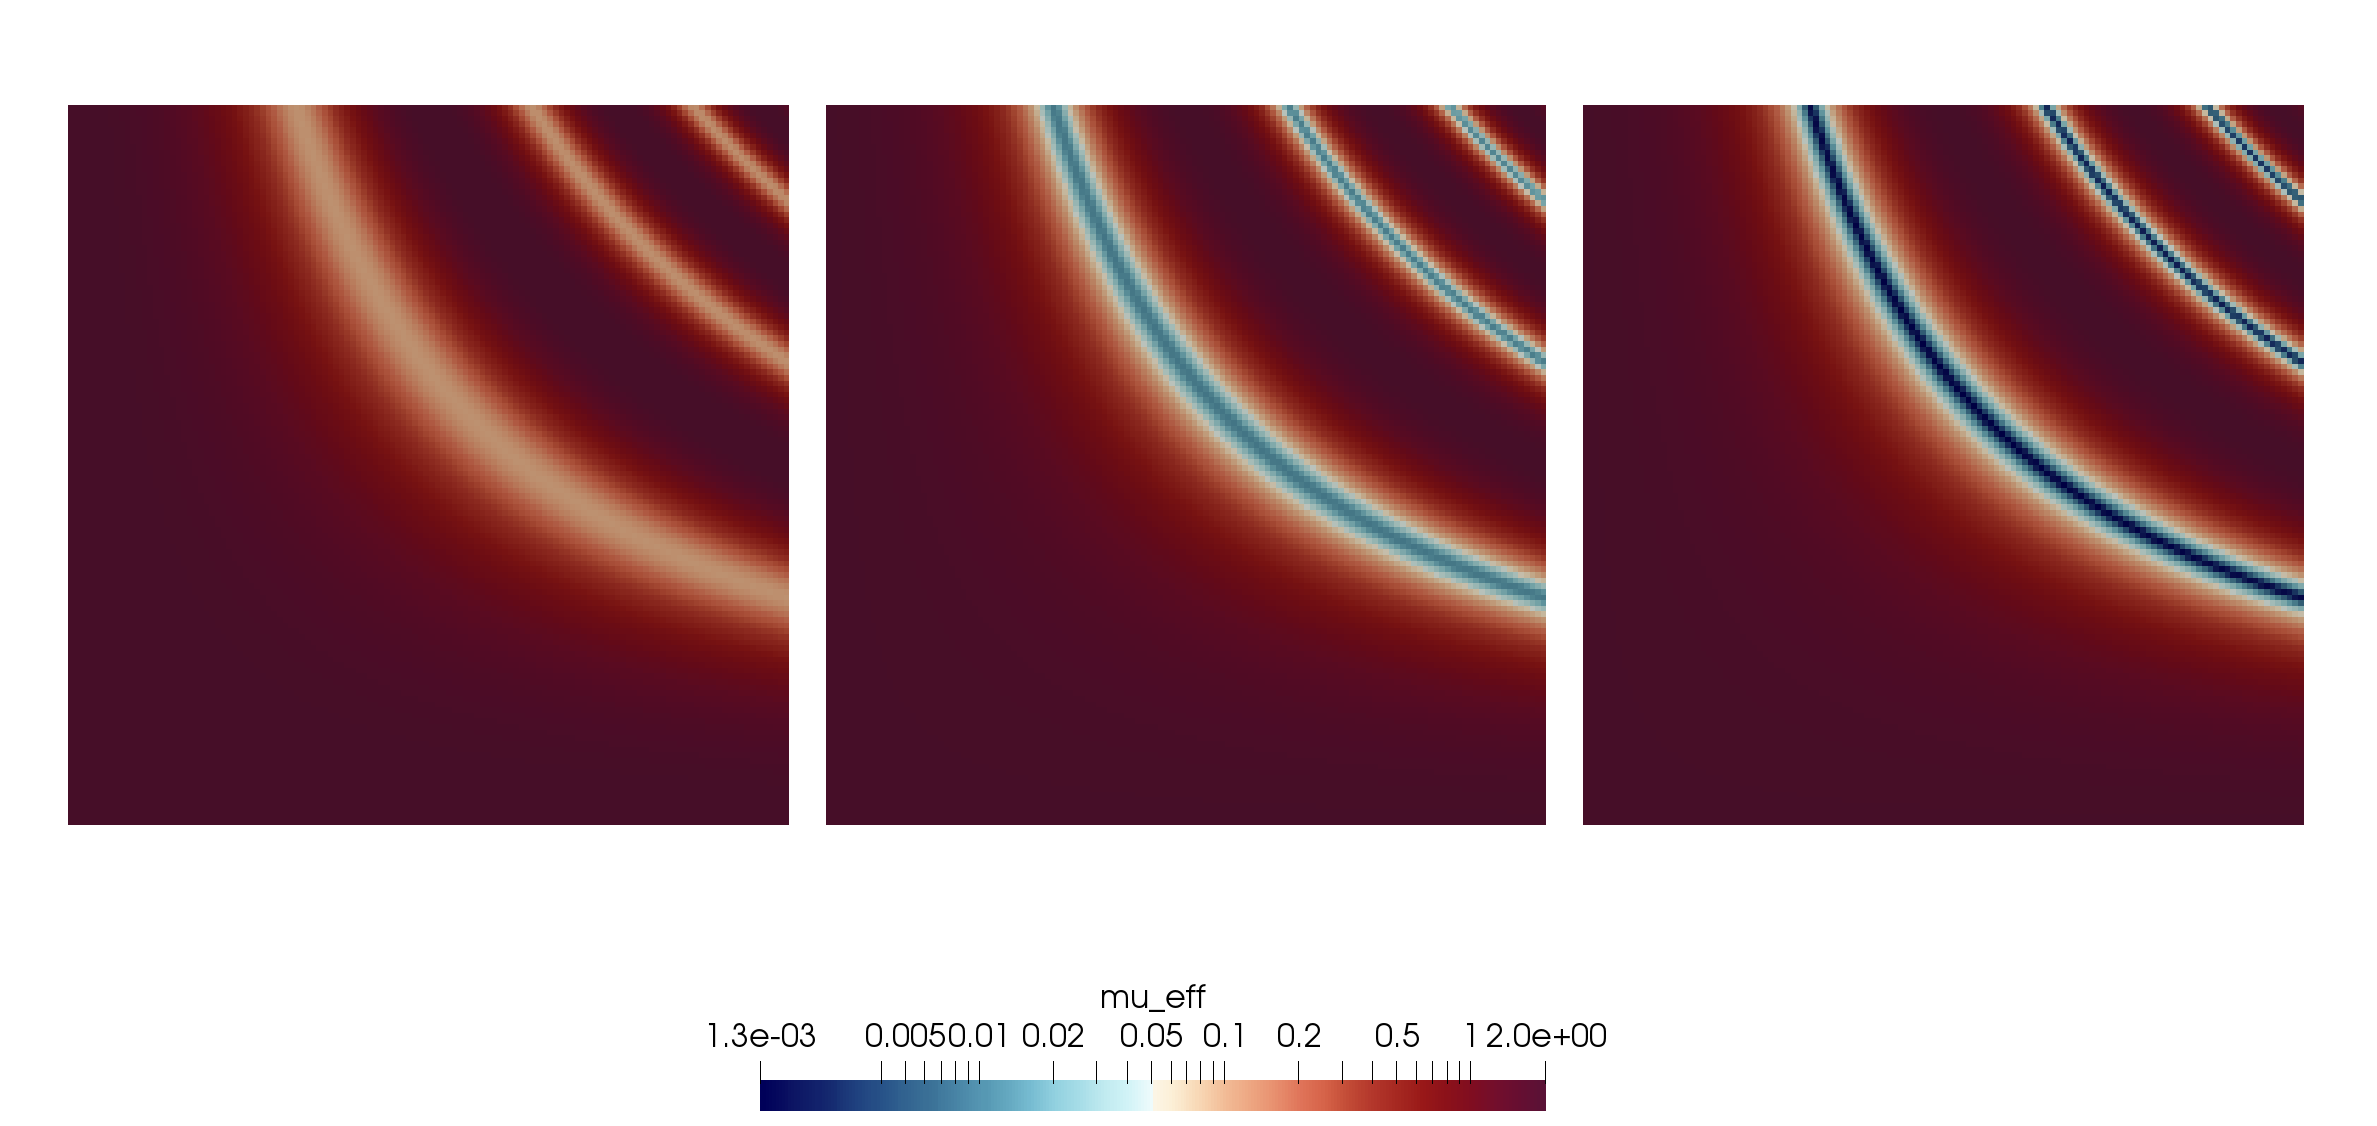
\includegraphics[width=14cm]{images/mms/mms7_mueffs}\\
Domain size 2x2 with $\epsilon=0.1, 0.01, 0.001$
\end{center}

Another interesting aspect of this benchmark is the fact that increasing the domain size
adds complexity to it as it increases the number of low viscosity zones and the spacing 
between them also decreases:

\begin{center}
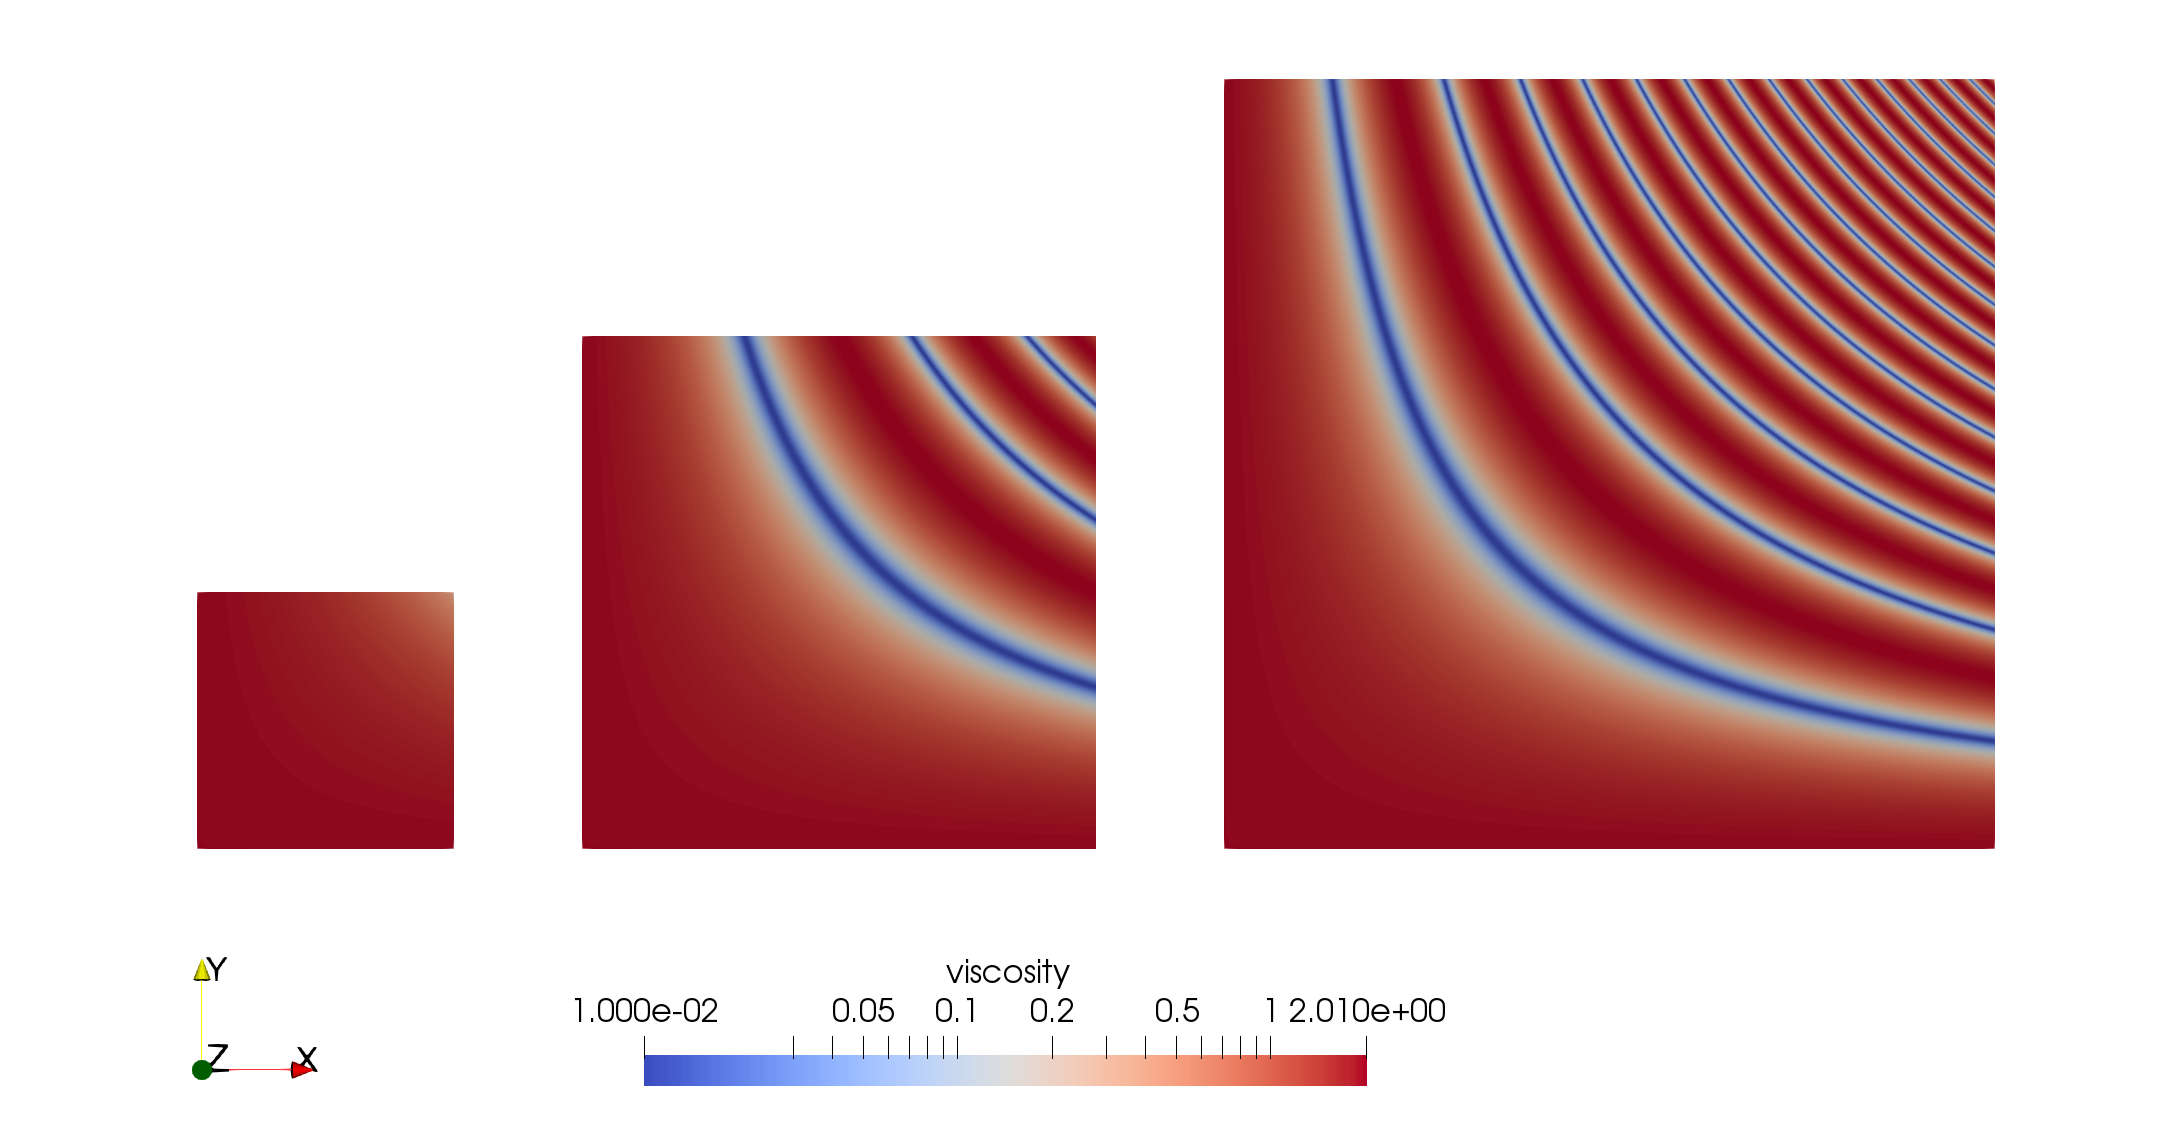
\includegraphics[width=7.28cm]{images/mms/mms7_visc}
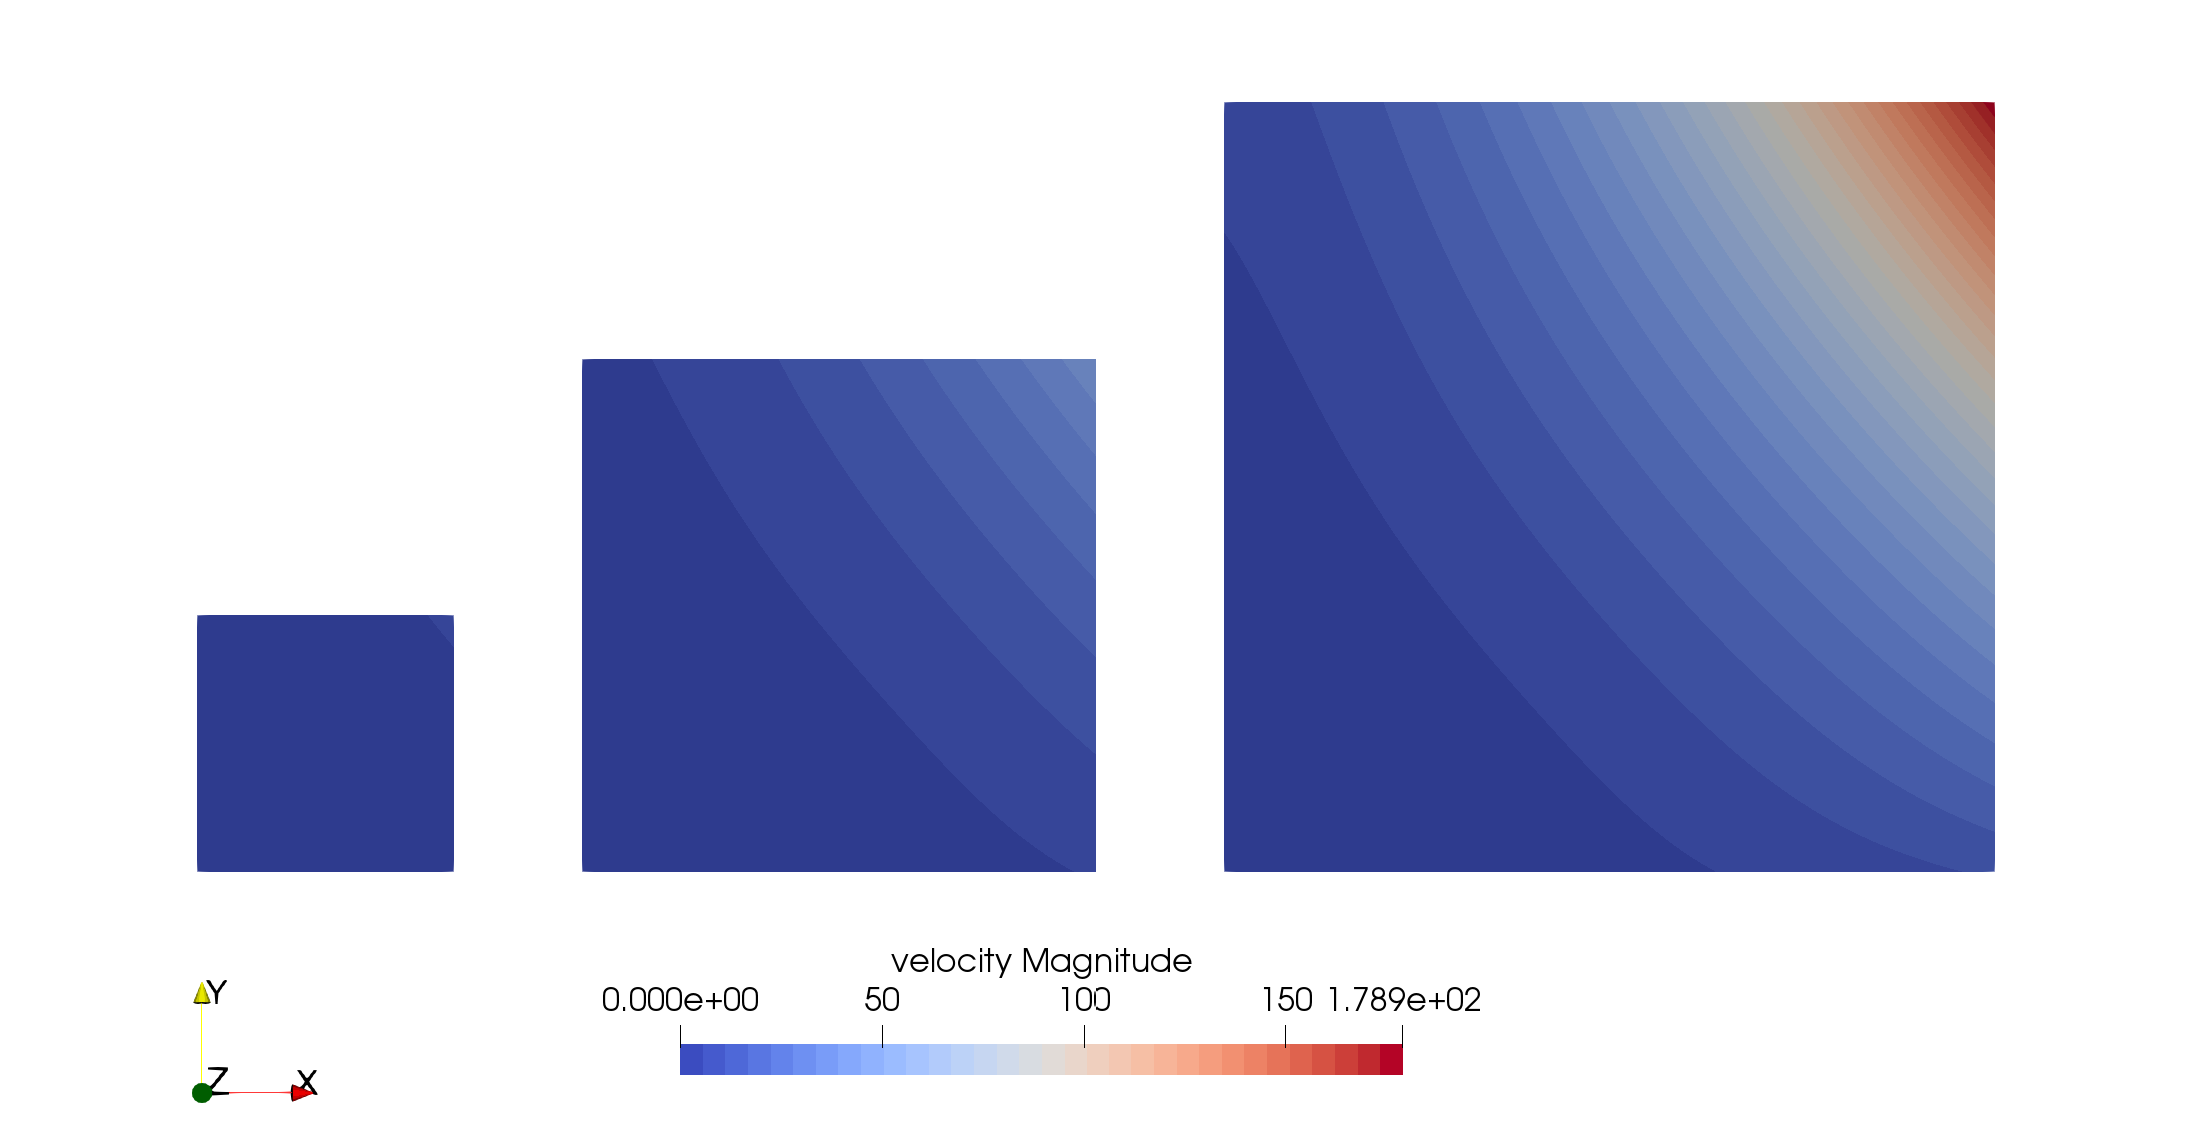
\includegraphics[width=7.28cm]{images/mms/mms7_vel}\\
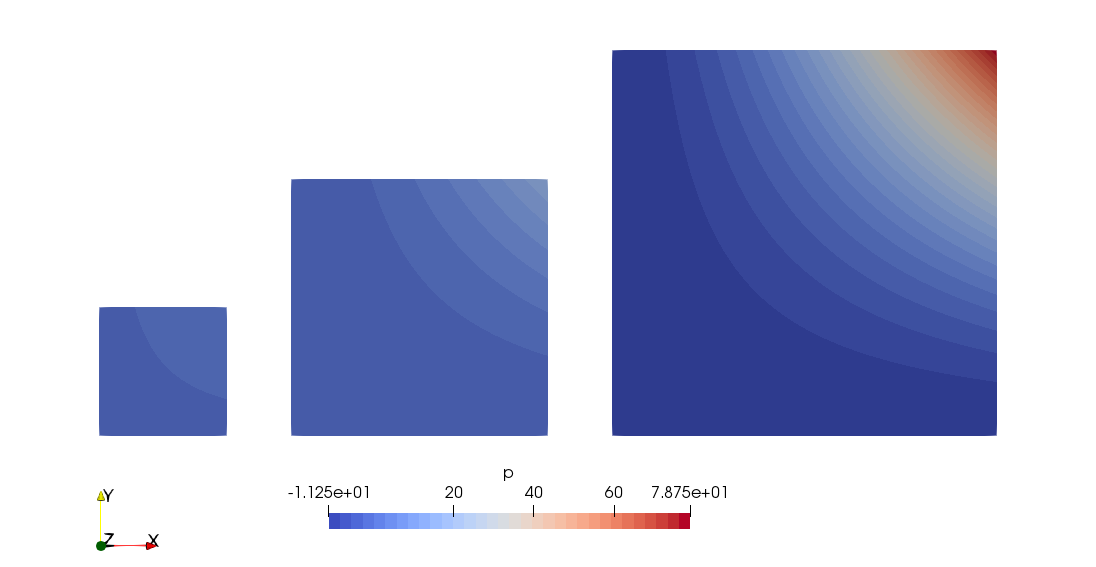
\includegraphics[width=7.28cm]{images/mms/mms7_press}
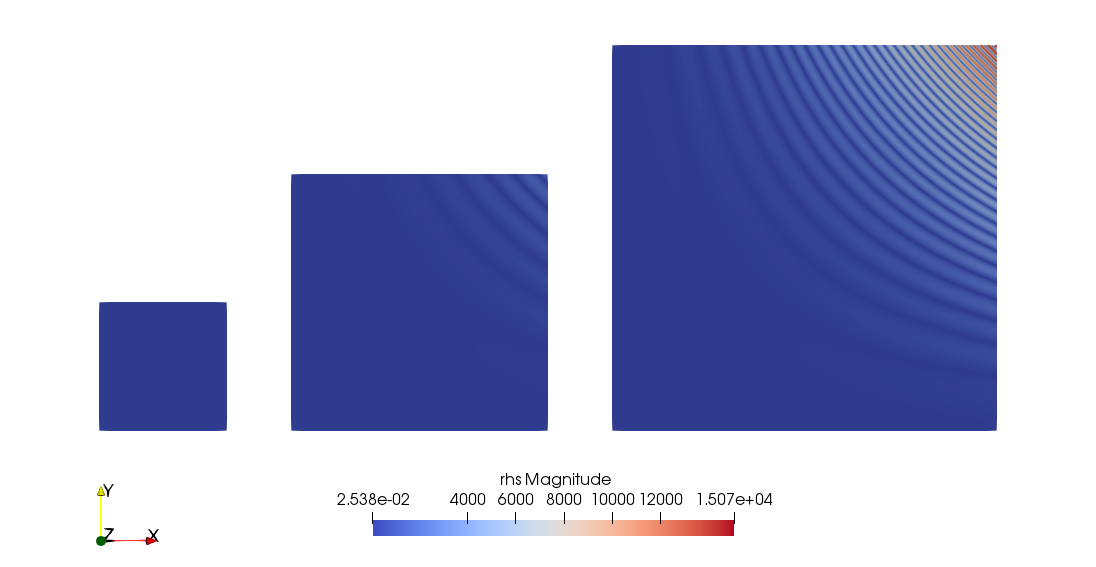
\includegraphics[width=7.28cm]{images/mms/mms7_rhs}\\
Three different domain sizes (1x1, 2x2, 3x3) with $\epsilon=0.001$.
\end{center}


Finally, because the analytical expression for both components of the velocity is a polynomial, we can also
compute the root mean square velocity exactly. For instance, for a 2x2 domain:
\begin{center}
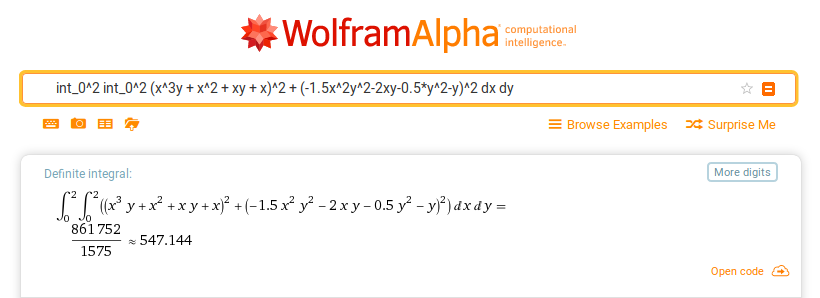
\includegraphics[width=8cm]{images/mms/mms7_vrmstheo}
\end{center}
and we end up with (for $L=2$)
\[
v_{rms} = \sqrt{\frac{1}{L^2}\frac{861752}{1575}} = \sqrt{\frac{215438}{1575}}
\simeq 11.6955560683
\]

I have added this benchmark to \aspect{}.
The velocity and pressure errors (in the $L_2$ norm) are measured for $L=1,2,3$, 
levels 3 to 9 (resolutions $8\times8$ to $512\times 512$)  
and $\epsilon=10^{-1},10^{-2},10^{-3}$. The figure below shows the velocity and pressure 
error convergence as a function of the mesh size for $\epsilon=0.1$ (results are identical for 
the other two $\epsilon$ values).
The expected convergence rates (cubic convergence for velocity and quadratic for pressure) are 
recovered for the $1\times 1$ domain at all resolutions. These rates are recovered for 
the $2\times 2$ domain for resolutions above level 6. We see that 
the multitude of low viscosity bands in the upper right corner of the $3\times 3$ domain 
will require a refinement level superior to 9 to recover the optimal convergence rates. 

\begin{center}
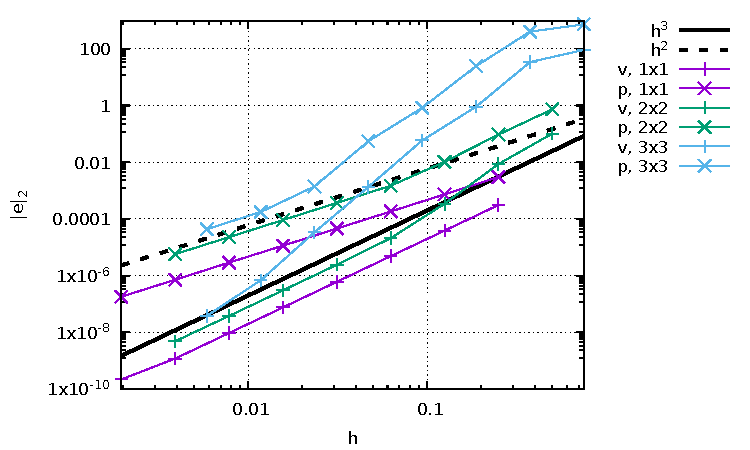
\includegraphics[width=7cm]{images/mms/mms7_errors}\\
{\captionfont Velocity and pressure error convergence as a function of the mesh size $h$ for 3 domain sizes with $\epsilon=0.1$.}
\end{center}

This benchmark is implemented and used in \stone~112.









